\section{Methodology}

\subsection{System Overview}
Figure~\ref{fig:system_overview} presents the system architecture. The user interacts through the interface, which captures video and displays feedback. The backend performs pose estimation, post-processing, and rep counting, then passes data to the feedback engine which returns results to the interface.

\begin{figure}[ht]
\centering
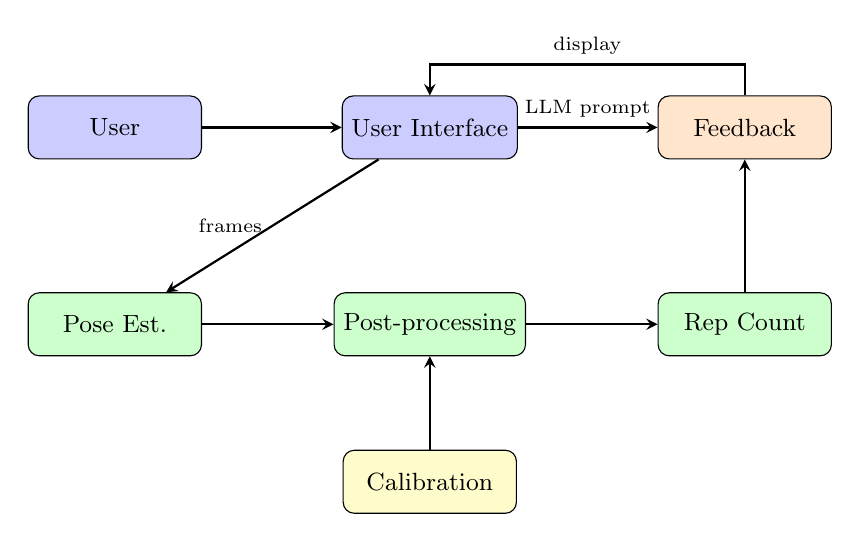
\begin{tikzpicture}[
    box/.style={rectangle, draw, rounded corners, minimum width=2.2cm, minimum height=0.8cm, align=center, font=\small},
    arrow/.style={->, >=stealth, thick}
]

% Top row: User flow
\node[box, fill=blue!20] (user) at (0,0) {User};
\node[box, fill=blue!20] (ui) at (4,0) {User Interface};
\node[box, fill=orange!20] (feedback) at (8,0) {Feedback};

% Bottom row: Processing pipeline
\node[box, fill=green!20] (pose) at (0,-2.5) {Pose Est.};
\node[box, fill=green!20] (filter) at (4,-2.5) {Post-processing};
\node[box, fill=green!20] (rep) at (8,-2.5) {Rep Count};

% Calibration below
\node[box, fill=yellow!20] (calib) at (4,-4.5) {Calibration};

% Arrows - top row
\draw[arrow] (user) -- (ui);
\draw[arrow] (ui) -- node[above,font=\scriptsize]{LLM prompt} (feedback);
\draw[arrow] (feedback) -- ++(0,0.8) -| node[pos=0.25,above,font=\scriptsize]{display} (ui);

% Arrows - UI to processing
\draw[arrow] (ui) -- node[left,font=\scriptsize]{frames} (pose);

% Arrows - processing pipeline
\draw[arrow] (pose) -- (filter);
\draw[arrow] (filter) -- (rep);
\draw[arrow] (rep) -- (feedback);

% Calibration arrow
\draw[arrow] (calib) -- (filter);

\end{tikzpicture}
\caption{FitCoachAR system architecture.}
\label{fig:system_overview}
\end{figure}

\subsection{Pose Acquisition}
We employ MediaPipe Pose \cite{lugaresi2019mediapipe} for real-time keypoint extraction (33 2D joints). The stream is smoothed using a One-Euro filter to reduce jitter and ensure sub-100 ms latency.


\subsection{Online Repetition Segmentation and Form Evaluation}

During live operation, repetition detection and form evaluation are decoupled but driven by
the same calibration parameters.

\paragraph{Repetition Detection.}
An online state machine operates on the primary signal and uses the calibrated thresholds
$\theta_{\text{low}}$ and $\theta_{\text{high}}$ to detect transitions between movement phases
(e.g., bottom, ascent, top, descent). A full traversal from bottom to top and back to bottom
is labeled as one repetition. This stage is intentionally form-agnostic and focuses solely on
robust cycle detection.

\paragraph{Form Check and Rep Acceptance.}
For each detected repetition, form metrics are evaluated against their calibrated normative
references. Given a live metric value $m$ and its normative reference $m_{\text{norm}}$, the
relative deviation is computed as:
\begin{equation}
    e = \frac{|m - m_{\text{norm}}|}{|m_{\text{norm}}|}.
\end{equation}

A user-controlled critic parameter $\delta$ scales the acceptable tolerance for all form
metrics. For a detected repetition to be considered \emph{valid}, every evaluated form
metric must satisfy the deviation constraint. Specifically, if there exists any metric
for which
\begin{equation}
    e > \delta,
\end{equation}
the repetition is marked as invalid and is not counted, even if the kinematic cycle was
successfully detected.

Only repetitions for which all form metrics satisfy $e \le \delta$ increment the repetition
counter.

\subsection{Feature Computation and Calibration}
From each repetition we compute angular features:
\begin{itemize}
    \item Active joints: elbows, knees, shoulders (max, min, correlation).
    \item Passive joints: spine and pelvis (mean, standard deviation).
\end{itemize}

During calibration, each key joint or motion phase $i$ is analyzed over three ``best-form'' repetitions:
The mean joint angle is
\begin{equation}
    \bar{U}_i = \frac{1}{3} \sum_{r=1}^{3} \theta_i^{(r)}
\end{equation}

Its deviation percentage from a canonical target $S_i$ is
\begin{equation}
    \eta_i = \frac{\\bar{U}_i - S_i}{S_i}
\end{equation}

The pair $(\bar{U}_i, \eta_i)$ forms the personalized baseline and offset for that user. Specifically, for Squats, the Knee Joint angle is calibrated to define the personalized depth threshold ($\theta_{depth}$). For Bicep Curls, the Elbow Joint angle is calibrated to define the full contraction threshold ($\theta_{peak}$). Other metrics (e.g., stability limits) rely on non-personalized biomechanical defaults to ensure safety.
During runtime, for each joint or phase, the system:
\begin{enumerate}
    \item Measures the current angle $\theta_i$
    \item Computes percentage deviation $e_i = \frac{|\theta_i - \bar{U}_i|}{|\bar{U}_i|}$
\end{enumerate}

A manually set critic parameter $\delta$ determines grading bands:
\begin{itemize}
    \item Good: $e_i < \delta$
    \item Relatively good: $\delta \le e_i < 1.2 \delta$
    \item Bad: $e_i \ge 1.2 \delta$
\end{itemize}

Repetition-level and session-level scores aggregate these joint/phase grades to summarize overall performance.


\subsection{FormScript: Interpretable Feedback via FormCodes}
\label{sec:formscript}

To provide meaningful, explanatory feedback, we implemented ``FormScript'', a rule-based system inspired by the ``PoseScript'' methodology \cite{delmas2022posescript}. The core problem is that simple rep counters don't tell users \textit{how} to improve---users need to know \textit{why} a rep was good or bad. FormScript solves this by discretizing continuous kinematic measurements into human-readable categories (FormCodes) and then applying logical production rules (Super FormCodes) to generate actionable feedback.

\subsubsection{FormCode Extraction and Categorization}

FormCodes are elementary descriptors that quantify specific aspects of body pose and motion. Each FormCode $c$ maps a continuous measurement $v \in \mathbb{R}$ to a discrete category $l \in \mathcal{L}_c$ based on predefined thresholds. We categorize FormCodes into two groups:

\begin{itemize}
    \item \textbf{Static FormCodes}: Evaluate body geometry on individual frames (e.g., joint angles, inter-joint distances, body segment orientations).
    \item \textbf{Dynamic FormCodes}: Evaluate motion quality over temporal windows (e.g., velocity, acceleration, stability deviations).
\end{itemize}

\paragraph{Measurement Computation}
FormCode measurements are derived from MediaPipe's 33-joint skeleton model. For static metrics, we compute:

\begin{itemize}
    \item \textbf{Joint Angles}: For a 3-joint chain $(a, b, c)$, the angle at joint $b$ is computed via the dot product of limb vectors.
    \item \textbf{Distances}: Euclidean distance between joint pairs, normalized by shoulder width for scale-invariance.
    \item \textbf{Orientations}: Pitch and roll angles of body segments (torso, pelvis) relative to vertical.
\end{itemize}

For dynamic metrics, we aggregate measurements over the duration of one repetition:

\begin{itemize}
    \item \textbf{Velocity}: Average rate of change of joint position or angle.
    \item \textbf{Jerk}: Rate of change of acceleration, quantifying smoothness.
    \item \textbf{Deviation}: Maximum displacement from expected trajectory.
\end{itemize}

\paragraph{Thresholding and Categorization}
Each FormCode defines categories via min/max thresholds. For example, squat depth categorizes knee angle $\theta$ as:
\begin{itemize}
    \item ``deep'' if $\theta \leq 90^\circ$
    \item ``parallel'' if $90^\circ < \theta \leq 110^\circ$
    \item ``shallow'' if $\theta > 110^\circ$
\end{itemize}

Thresholds incorporate noise tolerance ($\pm 5^\circ$ for angles, $\pm 0.05$ for normalized coordinates) to prevent spurious transitions. Exercise-specific FormCodes that depend on user range-of-motion (e.g., squat depth, bicep curl peak flexion) are dynamically adjusted using calibration data: the system measures the user's achievable range during a calibration phase and adapts thresholds accordingly (Section 3.3).

\subsubsection{Elementary FormCodes}

Following PoseScript's taxonomy, we define five types of elementary FormCodes. Each FormCode transforms a continuous measurement $v$ into a discrete category based on thresholds. Figure~\ref{fig:formscript-pipeline} illustrates the overall pipeline.

% Block diagram: FormScript Pipeline
\begin{figure}[ht]
\centering
\begin{tikzpicture}[
    node distance=1.2cm,
    block/.style={rectangle, draw, fill=blue!20, text width=2.2cm, text centered, rounded corners, minimum height=1cm},
    arrow/.style={thick,->,>=stealth}
]
% Nodes
\node[block] (video) {Video Frames};
\node[block, right=of video] (pose) {Pose Estimation};
\node[block, right=of pose, fill=red!30] (formcodes) {FormCodes};
\node[block, right=of formcodes, fill=red!30] (super) {Super FormCodes};
\node[block, right=of super] (analyzer) {Form Analyzer};
\node[block, below=0.8cm of analyzer] (llm) {LLM};
\node[block, left=of llm] (feedback) {Feedback};

% Arrows
\draw[arrow] (video) -- (pose);
\draw[arrow] (pose) -- (formcodes);
\draw[arrow] (formcodes) -- (super);
\draw[arrow] (super) -- (analyzer);
\draw[arrow] (analyzer) -- (llm);
\draw[arrow] (llm) -- (feedback);
\end{tikzpicture}
\caption{FormScript pipeline: video frames are processed through pose estimation, discretized into FormCodes, aggregated into Super FormCodes, analyzed, and converted to natural language feedback via LLM.}
\label{fig:formscript-pipeline}
\end{figure}

We categorize FormCodes into two groups based on their nature:

\begin{itemize}
    \item \textbf{Static FormCodes}: Evaluate body geometry (angles, distances, relative positions) on individual frames. While usually assessed at key moments for scoring (e.g., bottom of a squat), they can also be monitored continuously to detect persistent errors.
    \item \textbf{Dynamic FormCodes}: Evaluate motion quality over time (velocity, acceleration, stability) across a sequence of frames.
\end{itemize}

% Block diagram: FormCodes Hierarchy
\begin{figure}[ht]
\centering
\begin{tikzpicture}[
    node distance=1cm and 0.2cm,
    block/.style={rectangle, draw, text width=1.5cm, text centered, rounded corners, minimum height=0.6cm, font=\footnotesize},
    arrow/.style={thick,->,>=stealth}
]
% Top level
\node[block, fill=blue!20] (formcodes) {FormCodes};

% Second level
\node[block, fill=green!25, below left=1.2cm and 3cm of formcodes] (static) {Static};
\node[block, fill=orange!35, below right=1.2cm and 3cm of formcodes] (dynamic) {Dynamic};

% Static children (4 types)
\node[block, below=1.2cm of static, xshift=-1.5cm, fill=green!10] (angle) {Angle};
\node[block, right=0.1cm of angle, fill=green!10] (pitchroll) {Pitch/Roll};
\node[block, right=0.1cm of pitchroll, fill=green!10] (distance) {Distance};
\node[block, right=0.1cm of distance, fill=green!10] (relpos) {Rel. Pos.};

% Dynamic children (5 types)
\node[block, below=1.2cm of dynamic, xshift=-2cm, fill=orange!15] (velocity) {Velocity};
\node[block, right=0.1cm of velocity, fill=orange!15] (jerk) {Jerk};
\node[block, right=0.1cm of jerk, fill=orange!15] (deviation) {Deviation};
\node[block, right=0.1cm of deviation, fill=orange!15] (symmetry) {Symmetry};
\node[block, right=0.1cm of symmetry, fill=orange!15] (duration) {Duration};

% Arrows - top to second level
\draw[arrow] (formcodes.south) -- ++(0,-0.4) -| (static.north);
\draw[arrow] (formcodes.south) -- ++(0,-0.4) -| (dynamic.north);

% Arrows - Static to children
\draw[arrow] (static.south) -- ++(0,-0.4) -| (angle.north);
\draw[arrow] (static.south) -- ++(0,-0.4) -| (pitchroll.north);
\draw[arrow] (static.south) -- ++(0,-0.4) -| (distance.north);
\draw[arrow] (static.south) -- ++(0,-0.4) -| (relpos.north);

% Arrows - Dynamic to children
\draw[arrow] (dynamic.south) -- ++(0,-0.4) -| (velocity.north);
\draw[arrow] (dynamic.south) -- ++(0,-0.4) -| (jerk.north);
\draw[arrow] (dynamic.south) -- ++(0,-0.4) -| (deviation.north);
\draw[arrow] (dynamic.south) -- ++(0,-0.4) -| (symmetry.north);
\draw[arrow] (dynamic.south) -- ++(0,-0.4) -| (duration.north);
\end{tikzpicture}
\caption{FormCode hierarchy: Static (4 types) for spatial geometry; Dynamic (5 types) for temporal motion quality.}
\label{fig:formcode-taxonomy}
\end{figure}

\paragraph{Static FormCodes}

Static FormCodes analyze body geometry based on individual frames. While some are checked continuously (e.g., torso lean), others are critical at specific key moments (e.g., squat depth). We define five Static FormCode types:

\begin{itemize}
    \item \textbf{Angle}: Measure joint flexion (e.g., knee angle, elbow angle)
    \item \textbf{Distance}: Measure spacing between body parts (e.g., elbow-to-torso distance)
    \item \textbf{Relative Position}: Measure spatial relationships along X/Y/Z axes
    \item \textbf{Pitch \& Roll}: Measure body segment orientation relative to vertical
    \item \textbf{Ground Contact}: Detect contact with the ground
\end{itemize}

\paragraph{Dynamic FormCodes}

Dynamic FormCodes extend PoseScript's static approach to analyze motion quality over time, which is critical for exercise evaluation. We define five Dynamic FormCode types:

\begin{itemize}
    \item \textbf{Velocity}: Measure speed of movement phases (controlled, fast, explosive)
    \item \textbf{Jerk}: Measure smoothness via rate of acceleration change
    \item \textbf{Deviation}: Measure maximum displacement from expected trajectory
    \item \textbf{Symmetry}: Measure left-right asymmetry during movement
    \item \textbf{Duration}: Measure time spent in specific positions
\end{itemize}

Complete threshold definitions and categorization conditions for all FormCode types are provided in Appendix~\ref{appendix:formcodes}.

\subsubsection{Super FormCodes: Production Rules}

Super FormCodes aggregate multiple elementary FormCodes using logical production rules. Each Super FormCode defines a high-level body configuration by combining conditions with AND/OR operators.

\begin{table}[h]
\centering
\small
\begin{tabular}{|l|l|p{6cm}|}
\hline
\textbf{Subject} & \textbf{Configuration} & \textbf{Production Rule} \\
\hline
torso & upright & pitch \& roll (pelvis, L-shoulder) = vertical AND pitch \& roll (pelvis, R-shoulder) = vertical \\
\hline
body & bent forward & relativePos Y (L-ankle, neck) = below AND relativePos Z (neck, pelvis) = front \\
\hline
knees & deep squat & angle (L-knee) = completely bent AND angle (R-knee) = completely bent \\
\hline
knees & parallel squat & angle (L-knee) = bent at right angle AND angle (R-knee) = bent at right angle \\
\hline
knees & stable & distance (L-knee, L-foot) = close AND distance (R-knee, R-foot) = close \\
\hline
knees & collapsed & relativePos X (L-knee, L-foot) = at right of OR relativePos X (R-knee, R-foot) = at left of \\
\hline
elbows & anchored & distance (L-elbow, torso) = close AND distance (R-elbow, torso) = close \\
\hline
elbows & drifting & distance (L-elbow, torso) = spread OR distance (R-elbow, torso) = spread \\
\hline
feet & shoulder width & distance (L-foot, R-foot) = shoulder width AND pitch \& roll (L-foot, R-foot) = horizontal \\
\hline
\end{tabular}
\caption{Super FormCode production rules for exercise analysis.}
\label{tab:super-formcodes}
\end{table}

\subsubsection{Exercise-Specific FormCode Application}

\paragraph{Squat Analysis}
Key FormCodes monitored: knee angle (depth), torso pitch (lean), knee-to-foot distance (stability), hip levelness (asymmetry).

\paragraph{Bicep Curl Analysis}
Key FormCodes monitored: elbow angle (contraction), elbow-to-torso distance (anchoring), shoulder/hip pitch (swing detection), wrist angle (neutral grip).

\subsubsection{Configuration-Driven Definition}

A key strength of the FormScript framework is its extensibility. Rather than hard-coding rules, all FormCodes and Super FormCodes are defined in external configuration files, making it easy for domain experts (e.g., physiotherapists) to adjust thresholds or add new exercises without modifying the core codebase.

\paragraph{Elementary Configuration}
FormCodes are defined by specifying the measurement type and categorization thresholds. Table~\ref{tab:formcode_example} shows an example configuration for squat depth.

\begin{table}[ht]
\centering
\small
\begin{tabular}{llc}
\toprule
\textbf{Category} & \textbf{Threshold} & \textbf{Interpretation} \\
\midrule
deep & $\theta < 90^\circ$ & Full depth squat \\
parallel & $90^\circ \leq \theta < 110^\circ$ & Thighs parallel \\
shallow & $\theta \geq 110^\circ$ & Insufficient depth \\
\bottomrule
\end{tabular}
\caption{Example FormCode: \texttt{squat\_depth} (knee angle).}
\label{tab:formcode_example}
\end{table}

\paragraph{Production Rule Configuration}
Super FormCodes combine elementary FormCodes using logical rules. Table~\ref{tab:superformcode_example} shows an example for detecting a good squat repetition.

\begin{table}[ht]
\centering
\small
\begin{tabular}{lll}
\toprule
\textbf{FormCode} & \textbf{Must Be} & \textbf{Must Not Be} \\
\midrule
squat\_depth & deep & --- \\
knee\_stability & --- & unstable, wobble \\
torso\_angle & --- & bent\_over, leaning \\
\bottomrule
\end{tabular}
\caption{Example Super FormCode: \texttt{GOOD\_REP} rule definition.}
\label{tab:superformcode_example}
\end{table}

This data-driven approach decouples the biomechanical definitions from the pose estimation logic, similar to the PoseScript architecture \cite{delmas2022posescript}.

\subsubsection{Feedback Systems}

The FormScript pipeline feeds into two complementary feedback paths: real-time coaching during exercise and offline analysis after workout completion.

\paragraph{Real-Time Feedback}
During exercise, feedback must maintain sub-100ms latency. The repetition counter tracks four phases: BOTTOM $\rightarrow$ UP\_PHASE $\rightarrow$ TOP $\rightarrow$ DOWN\_PHASE. The system provides:

\begin{enumerate}
    \item \textbf{Intra-Rep Guidance}: During the UP\_PHASE (before the rep is counted), the system monitors form and provides corrective cues to help users complete each repetition properly:
    \begin{itemize}
        \item ``Go deeper!'' --- when squat depth is insufficient to reach TOP
        \item ``Keep elbows still!'' --- when elbow drift is detected during curl ascent
        \item ``Knees out!'' --- when knee cave is forming during squat ascent
    \end{itemize}
    
    \item \textbf{Post-Rep Summary}: After each repetition completes (reaching BOTTOM again), Super FormCodes trigger brief feedback:
    \begin{itemize}
        \item GOOD\_REP $\rightarrow$ ``Nice rep!''
        \item BODY\_SWING $\rightarrow$ ``Less swing next time''
    \end{itemize}
    
    \item \textbf{Guidance Arrows}: Visual AR overlays on the skeleton showing direction of correction:
    \begin{itemize}
        \item Arrow on wrist pointing up for INCOMPLETE\_RANGE
        \item Arrow on knee pointing outward for KNEE\_CAVE
        \item Arrow on hip pointing down for SHALLOW\_SQUAT
    \end{itemize}
\end{enumerate}

\paragraph{Offline Feedback (Post-Workout)}
After the workout session, accumulated FormCode data from all repetitions is processed for comprehensive analysis:

\begin{enumerate}
    \item \textbf{Per-Rep Feedback Generation}: Each repetition's FormCodes are converted to human-readable sentences. For example:
    \begin{itemize}
        \item peak\_flexion = full\_contraction $\rightarrow$ ``You achieved a full muscle contraction at the top of the curl.''
        \item swing\_momentum = body\_swing $\rightarrow$ ``Significant body swing detected---you're using momentum instead of muscle.''
    \end{itemize}
    
    \item \textbf{LLM-Powered Session Summary}: An aggregated session summary is sent to an LLM (Llama 3.3 70B via Cerebras). The summary contains: total reps, good reps count, form score percentage, the top 2 detected issues with their Super FormCode names and descriptions, and \textbf{all per-rep FormScript feedback sentences}. These requests are logged to \texttt{llm\_logs/} for debugging. The LLM generates a natural language summary with:
    \begin{itemize}
        \item Positive acknowledgment of effort
        \item Form score and rep count
        \item Constructive tip for the most common issue
        \item Motivation for next session
    \end{itemize}
    
    \item \textbf{Q\&A Capability}: Users can ask follow-up questions about their workout (e.g., ``How was my elbow position?'') and receive personalized responses based on their session data.
\end{enumerate}

This dual-path approach ensures users receive immediate, actionable feedback during exercise while benefiting from comprehensive LLM-generated insights after workout completion.

\subsubsection{Feedback Hierarchy and Prioritization}
To manage user cognitive load and maximize learning efficiency, we employ a multi-tiered feedback strategy:

\paragraph{Real-Time Prioritization}
During the exercise, the user's attention is limited. Displaying multiple simultaneous errors can be overwhelming. Therefore, the Real-Time Coach uses a \textit{priority queue} strategy. Errors are checked in a hierarchical order based on safety and mechanical importance (e.g., ``Elbow Stability'' $>$ ``Range of Motion''). The system halts at the first detected error and generates only that specific feedback command and AR arrow. This ensures the user focuses on correcting the most critical flaw before optimizing secondary aspects.

\paragraph{Post-Set Frequency Ranking}
Conversely, the post-workout analysis aggregates data from the entire session. Here, completeness is preferred over simplicity. The system counts all detected FormCodes across all repetitions and ranks them by frequency. The top-ranked issues are presented in the summary, allowing users to identify persistent habits or muscle imbalances that require long-term attention.

\paragraph{Feedback Stability}
Real-time pose estimation can exhibit minor jitter, potentially causing the feedback state to flicker when the user's form is near a decision threshold. To address this, we implemented a temporal hysteresis mechanism. Once an error is detected, the corresponding AR feedback is ``locked'' for a minimum duration of 0.5 seconds (15 frames). This ensures the user has sufficient time to perceive and react to the guidance, preventing visual instability.

